%!TEX root = ../effc_top.tex

\begin{frame}{Operations at odd primes}
	\pause
	Steenrod squares from derived commutativity of \textbf{binary} product.

	\bigskip\pause
	Steenrod also defined operations (for $\beta \in \{0,1\}$)
	\[
	\beta^{\varepsilon} P_k \colon H^\bullet(X; \Fp) \to H^\bullet(X; \Fp)
	\]
	from derive commutativity of higher arity product.

	\bigskip\pause
	Organized by $E_\infty$-structures\pause, which have a long history:
	\begin{itemize}
		\item (co)homology operations, \pause
		\item recognition of infinite loop spaces, \pause
		\item algebraic models of the homotopy category.
	\end{itemize}
\end{frame}

\begin{frame}{An $E_\infty$-coalgebra on chains}
	\pause
	\textcolor{pblue}{Theorem (Med.)} \\
	The collection of maps $\gchains(\gsimplex^n) \to \gchains(\gsimplex^n)^{\otimes r}$ obtained from compositions of
	\begin{align*}
		\Delta &\colon \gchains(\gsimplex^n) \to \gchains(\gsimplex^n)^{\otimes 2}
		\qquad \text{(AW diagonal)} \\
		\ast &\colon \gchains(\gsimplex^n)^{\otimes 2} \to \gchains(\gsimplex^n)
		\qquad \text{(Join map)}
	\end{align*}
	defines an $E_\infty$-coalgebra on simplicial chains.

	\bigskip\pause
	\textcolor{pblue}{Example} \\
	\qquad\qquad \scalebox{0.7}{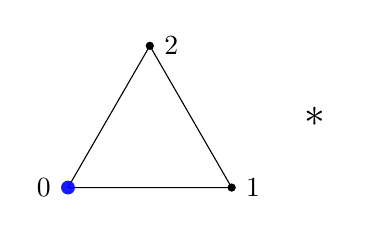
\begin{tikzpicture}[scale=.6]
\coordinate (A) at (210:2);
\coordinate (B) at (-30:2);
\coordinate (C) at (90:2);

\draw[draw=black] (A) -- (B) -- (C) -- (A);

\node[circle,fill=blue, opacity=.9, inner sep=0pt,minimum size=5pt, label=left:{0}] (a) at (A) {};
\node[circle,fill=black,inner sep=0pt,minimum size=3pt, label=right:{$1$}] (a) at (B) {};
\node[circle,fill=black,inner sep=0pt,minimum size=3pt, label=right:{$2$}] (a) at (C) {};

\node[scale=1.5] at (3.5,0.5) {$\ast$};
\end{tikzpicture}
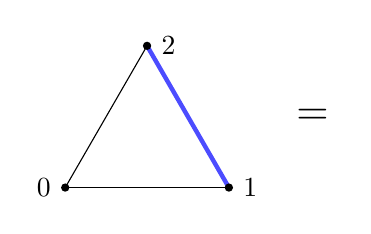
\begin{tikzpicture}[scale=.6]
\coordinate (A) at (210:2);
\coordinate (B) at (-30:2);
\coordinate (C) at (90:2);

\draw[draw=blue,  ultra thick, draw opacity=.7] (B) -- (C);
\draw[draw=black] (C) -- (A);
\draw[draw=black] (A) -- (B);

\node[circle,fill=black,inner sep=0pt,minimum size=3pt, label=left:{$0$}] (a) at (A) {};
\node[circle,fill=black,inner sep=0pt,minimum size=3pt, label=right:{$1$}] (a) at (B) {};
\node[circle,fill=black,inner sep=0pt,minimum size=3pt, label=right:{$2$}] (a) at (C) {};

\node[scale=1.5] at (3.5,.5) {=};
\end{tikzpicture}
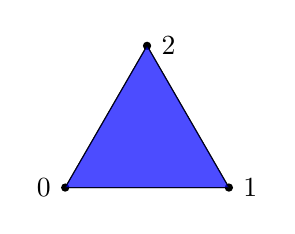
\begin{tikzpicture}[scale=.6]
\coordinate (A) at (210:2);
\coordinate (B) at (-30:2);
\coordinate (C) at (90:2);

\draw[draw=black] (A) -- (B) -- (C) -- (A);

\node[circle,fill=black,inner sep=0pt,minimum size=3pt, label=left:{$0$}] (a) at (A) {};
\node[circle,fill=black,inner sep=0pt,minimum size=3pt, label=right:{$1$}] (a) at (B) {};
\node[circle,fill=black,inner sep=0pt,minimum size=3pt, label=right:{$2$}] (a) at (C) {};

\draw[draw, fill=blue, opacity=.7] (A) -- (B) -- (C) -- (A);
\end{tikzpicture}}

	\bigskip\pause
	Also, versions for: \par
		\qquad \textcolor{pblue}{cubical} (Kaufmann--Med.) and \par
		\qquad \textcolor{pblue}{multisimplicial} (Med.--Pizzi--Salvatore) chains.
\end{frame}

%\begin{frame}{Two $E_\infty$-bialgebra models for loop spaces}
%	\pause
%	Based space $(X,x)$ $\rightarrow$ ``topological monoid'' $\Omega_x X$
%
%	\medskip\pause
%	Cubical singular chains define $\rS^{\square}(\Omega_x X)$ a monoid in $\mathsf{Ch}$.
%
%	\medskip\pause
%	Adams cobar construction applied to based singular chains $\mathbb{\Omega} \rS^{\triangle}(X, x)$:
%
%\end{frame}

\begin{frame}[fragile]{Two $E_\infty$-bialgebra models for loop spaces}
	\pause
	\textcolor{pblue}{Adams}:
	\vspace*{-11pt}
	\begin{center}
		Based space $(X,x)$ \\ \pause
		$\Downarrow$ \\
		``Topological monoid'' $\Omega_x X$ \\ \pause
		$\Downarrow$ \\
		Two algebras
		and a q-iso of algebras: \\
		\medskip
		$\mathbb{\Omega} \rS^{\triangle}(X, x)$
		$\xra{\ \theta_X\ }$
		$\rS^{\square}(\Omega_x X)$
	\end{center}

	\bigskip\pause
	\textcolor{pblue}{Baues}:
	\vspace*{-11pt}
	\begin{center}
		$\theta_X$ is a map of monoids in $\mathsf{coAlg}$
	\end{center}

	\bigskip\pause
	\textcolor{pblue}{Med.--Rivera}:
	\vspace*{-11pt}
	\begin{center}
		$\theta_X$ is a map of monoids in $\mathsf{coAlg}_{E_\infty}$
	\end{center}

%	\medskip\pause
%	\begin{theorem}[Med.--Rivera]
%		$\theta_X$ is a q-iso of monoid in $\mathsf{coAlg}_{E_\infty}$
%	\end{theorem}
\end{frame}

\begin{frame}[fragile]{May--Steenrod structures}

	\vskip-5pt\pause

	\begin{block}{Construction (Kaufmann-Med.)}
		Explicit cup-$(p,i)$ coproducts defining \textcolor{pblue}{operations} on $H^\bullet(-; \Fp)$.
	\end{block}

	\pause

	\begin{block}{Implementation (Med.)}
		In the computer algebra system \textcolor{pblue}{\texttt{ComCH}}.
	\end{block}

	\pause

	For example, $\Delta_{3,2}[0,1,2]$ is equal to

	\begin{verbatim}
		- [0,1][0,1,2][0,1] + [0,1,2][0,2][0,1] + [0,2][0,2][0,1,2]
		- [0,1,2][0,1,2][1] - [0,2][0,1,2][1,2] + [0,1,2][1,2][1,2]
		- [0,1][1,2][0,1,2] - [0,1,2][2][0,1,2] - [0][0,1,2][0,1,2]
	\end{verbatim}

	\pause

	\textcolor{pblue}{Future directions:} (from the even to odd primes)

	\pause
	\begin{enumerate}
		\item Faster implementations for use in TDA. \pause \\
		\item Relation to higher category theory. \pause \\
		\item Connections to convex geometry. \pause \\
		\item Cartan and Adem coboundaries. \pause \\
		\item Where are these used in physics?
	\end{enumerate}
\end{frame}